\documentclass{beamer}

\usepackage{mathtools}
\usepackage{tikz}
\usepackage{pgfplots}
\usetikzlibrary{calc,positioning,arrows,decorations.markings}
\pgfplotsset{compat=1.14}

% --------------------------------------------------------- continue number counter over multiple slides
\usepackage{enumitem}
\setenumerate[1]{label=\arabic*.}

\setitemize{label=\usebeamerfont*{itemize item}%
  \usebeamercolor[fg]{itemize item}
  \usebeamertemplate{itemize item}}

\newcounter{ResumeEnumerate}

% --------------------------------------------------------- x'ed out arrow
\newcommand*{\StrikeThruDistance}{0.2cm}%
\newcommand*{\StrikeThru}{\StrikeThruDistance,\StrikeThruDistance}%
\tikzset{
  strike thru arrow/.style={
    decoration={
      markings, mark=at position 0.5 with {
        \draw [red, very thick, solid,-] ++ (-\StrikeThruDistance,-\StrikeThruDistance) -- ( \StrikeThruDistance, \StrikeThruDistance);
        \draw [red, very thick, solid,-] ++ (-\StrikeThruDistance,\StrikeThruDistance) -- (\StrikeThruDistance, -\StrikeThruDistance);
      }
    },
    postaction={decorate},
  }
}

% --------------------------------------------------------- abbrev
\newcommand{\goedel}[1]{\langle #1 \rangle}
\newcommand{\nats}{\mathbb{N}}
\newcommand{\reals}{\mathbb{R}}
\newcommand{\ints}{\mathbb{Z}}

\newcommand{\setup}{\textbf{SETUP} }
\newcommand{\asign}{\textbf{ASIGN} }
\newcommand{\averify}{\textbf{AVERIFY} }
\newcommand{\verify}{\textbf{VERIFY} }
\newcommand{\keygen}{\textbf{KGEN}}

\newcommand{\mespace}{\mathcal{M}}
\newcommand{\sspace}{\mathcal{S}}
\newcommand{\uspace}{\mathcal{U}}
\newcommand{\kspace}{\mathcal{K}}
\newcommand{\kfspace}{\mathcal{F}}


% --------------------------------------------------------- beamer/document setup
\mode<presentation>

\title{Concurrent Signatures}
% \subtitle{subtitle}

\author{Samir Benzammour}
\date{24th March 2020}
 
\institute[RWTH]{
  Algorithms and Computational Complexity\\
  RWTH Aachen University
}

% fonts etc
\usetheme{Madrid}
\usecolortheme{default}
\usefonttheme{professionalfonts}

\AtBeginSection[]
{
  \begin{frame}
    \frametitle{Outline}
    \tableofcontents[currentsection]
  \end{frame}
}

% \AtBeginSubsection[]
% {
%   \begin{frame}
%     \frametitle{Outline}
%     \tableofcontents[currentsubsection]
%   \end{frame}
% }

\begin{document}


\frame{\titlepage}

% --------------------------------------------------------- Global
\begin{frame}
	\frametitle{Outline}
	\tableofcontents
\end{frame}

% --------------------------------------------------------- Introduction
\section{Introduction}
\begin{frame}
	\frametitle{Security Model}

	\begin{itemize}
		\item Security is formalized through different key aspects.
		\item e.g. in Ring Signatures one property is \textcolor{red}{xyz}
	\end{itemize}

	And why are they important for our signature scheme?\\
	~\\
	Parallel to this, present an example to illustrate the different key points (maybe using secondary beamer for this)
\end{frame}

\subsection{Concurrent Approach}
\begin{frame}
	\frametitle{Concurrent Approach}
	
	\begin{itemize}
		\setlength\itemsep{1em}
		\item A and B sign messages $M_A$ and $M_B$ respectively
		\item identity is arbitrary \textcolor{blue}{signature ownership not derivable at this point}
		\item commitment upon release of \textit{keystone k}
		\item 
	\end{itemize}
\end{frame}

% --------------------------------------------------------- Preliminaries
\section{Preliminaries}
% \begin{frame}
	\frametitle{Security Model}

	\begin{itemize}
		\item Security is formalized through different key aspects.
		\item e.g. in Ring Signatures one property is \textcolor{red}{xyz}
	\end{itemize}

	And why are they important for our signature scheme?\\
	~\\
	Parallel to this, present an example to illustrate the different key points (maybe using secondary beamer for this)
\end{frame}

\subsection{Discrete Logarithm Assumption}
\begin{frame}
	\frametitle{Discrete Logarithmic Assumption}

	\begin{definition}[discrete logarithm]
		\begin{itemize}
			\item Group $\mathbb{G}$ given
			\item $b^k$ always defined in $\mathbb{G}$ through $b^k = \underbrace{b\cdot b \cdots b}_{k\text{ times}}$
			\item the \textbf{discrete logarithm} is an integer $k$, such that $b^k = a$
		\end{itemize}
	\end{definition}
	\begin{block}{Notation}
		\begin{itemize}
			\item Let $\mathcal{G}$ be a function generating a group
			\item Let $\mathcal{A}$ be a given algorithm
			\item Let $||\cdot||$ be the bit-length of a given integer
		\end{itemize}
	\end{block}
	\textcolor{red}{include definition of a generator?}
\end{frame}

\begin{frame}
	\frametitle{Discrete Logarithmic Assumption}
	\begin{block}{Discrete-Logarithm Experiment $DLog_{\mathcal{A}, \mathcal{G}}(n)$} % consider this experiment with
		\begin{itemize}
			\item Run $\mathcal{G}(1^n)$ to acquire $(\mathbb{G}, q, g)$ where $\mathbb{G}$ is a group, $q$ is its order (whereas $||q|| = n$) and $g\in \mathbb{G}$ is $\mathbb{G}$'s generator
			\item Choose a random $h\in\mathbb{G}$
			\item $\mathcal{A}$ is given $\mathbb{G}, q, g$ and $h$, and outputs $i\in \mathbb{Z}_p$ \textcolor{red}{define what $\mathbb{Z}_p$ is?}
			\item The result of the experiment is $1$ if $g^i = h$, and $0$ otherwise.
		\end{itemize}
	\end{block}
	\begin{definition}
		We say the \textbf{discrete logarithm problem is hard relative to} $\mathcal{G}$ if for all polynomial-time algorithms $\mathcal{A}$ there exists a negligible function $\textsf{negl}$ such that 
			$$\Pr[DLog_{\mathcal{A}, \mathcal{G}}(n) = 1] \leq \textsf{negl}(n)$$
	\end{definition}
\end{frame}

\subsection{Random Oracle}
\begin{frame}
	\frametitle{Random Oracle}

	\begin{block}{Definition (Oracle)}
		An \textbf{oracle} (machine) is an abstract machine that takes an input and generates a solution for it without knowing its inner workings.
	\end{block}
	\begin{block}{Definition (Random Oracle)}
		A \textbf{random oracle} is a oracle, which fulfills the following properties
		\begin{itemize}
			\item returns each \textit{unique} request with a truly random value (chosen from output domain)
			\item repeated requests (always) return the same response
		\end{itemize}
	\end{block}
\end{frame}

\subsection{Definitions}
\begin{frame}
	\frametitle{Definitions}
\end{frame}

% --------------------------------------------------------- Concurrent Signature Protocol
\section{Concurrent Signature Protocol}
\begin{frame}
	\frametitle{Security Model}

	\begin{itemize}
		\item Security is formalized through different key aspects.
		\item e.g. in Ring Signatures one property is \textcolor{red}{xyz}
	\end{itemize}

	And why are they important for our signature scheme?\\
	~\\
	Parallel to this, present an example to illustrate the different key points (maybe using secondary beamer for this)
\end{frame}

% --------------------------------------------------------- Security Model
\section{Security Model}
\begin{frame}
	\frametitle{Security Model}

	\begin{itemize}
		\item Security is formalized through different key aspects.
		\item e.g. in Ring Signatures one property is \textcolor{red}{xyz}
	\end{itemize}

	And why are they important for our signature scheme?\\
	~\\
	Parallel to this, present an example to illustrate the different key points (maybe using secondary beamer for this)
\end{frame}

\subsection{Unforgeability}
\begin{frame}
	\frametitle{Unforgeability}

	\begin{itemize}
		\item consider adversary $E$ and challenger $C$
		\item $C$ runs \setup
		\item $E$ acquires all public variables, $C$ retains all $x_i$
		\item $E$ can request\\[.2cm]
			$\left.\parbox{.5\textwidth}{%
			\begin{itemize}
				\item \textbf{KGen\ldots}
				\item \textbf{KReveal\ldots}
				\item \textbf{ASign\ldots} 
				\item \textbf{AVerify / Verify\ldots}
				\item \textbf{Private Key Extraction\ldots}
			\end{itemize}%
			}\right\}\text{\ldots Queries from } C$
		\item $E$ wins if \textcolor{blue}{$\averify = accept$} and no Private Key Extraction Query was made
		\end{itemize}
\end{frame}

\subsection{Ambiguity}
\begin{frame}
	\frametitle{Ambiguity}

  	
  \begin{center}
    \resizebox{.95\hsize}{!}{
      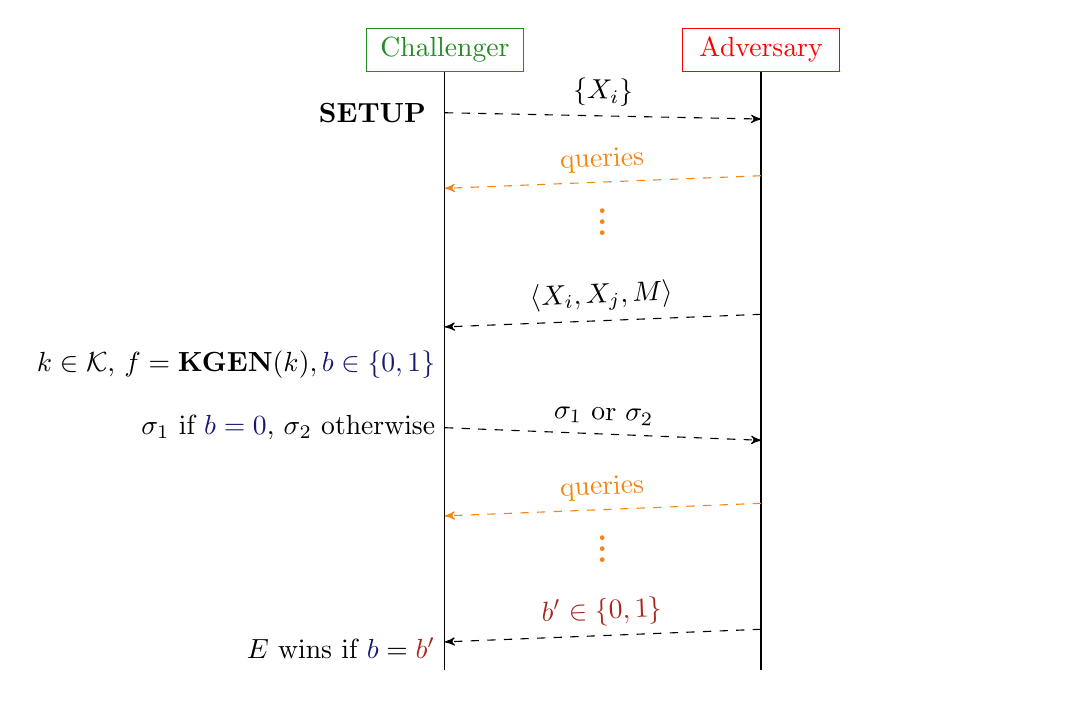
\begin{tikzpicture}[node distance=2cm,auto,>=stealth']
        \node[draw, minimum width = 2cm, color=Red] (adversary) {Adversary};
        \node[draw, minimum width = 2cm, color=ForestGreen, left = of adversary] (challenger) {Challenger};
        \node[below of=adversary, node distance=8cm] (adversaryground) {};
        \node[below of=challenger, node distance=8cm] (challengerground) {};
        
        % vertical lines
        \draw (challenger) -- (challengerground);
        \draw (adversary) -- (adversaryground);
      
        % setup
        \node[left, align=left] at ($(challenger)!0.1!(challengerground)$) {\setup};
        \visible<2->{\draw[->, dashed] ($(challenger)!0.1!(challengerground)$) -- node[sloped, above]{$\{X_i\}$} ($(adversary)!0.11!(adversaryground)$);}
        
        \visible<3->{\draw[->, dashed, BurntOrange] ($(adversary)!0.2!(adversaryground)$) -- node[sloped, above] (queries0) {queries} ($(challenger)!0.22!(challengerground)$);}
        \visible<3->{\node[below = 0mm of queries0, black] {\huge \textcolor{BurntOrange}{$\vdots$}};}

        \visible<4->{\draw[->, dashed] ($(adversary)!0.42!(adversaryground)$) -- node[sloped, above]{$\goedel{X_i, X_j, M}$} ($(challenger)!0.44!(challengerground)$);}

        \visible<5->{\node[left, align=left] at ($(challenger)!0.5!(challengerground)$) {$k\in\kspace$, $f = \textbf{KGEN}(k), \textcolor{MidnightBlue}{b\in\{0,1\}}$};}
        \visible<6->{\node[left, align=left] at ($(challenger)!0.6!(challengerground)$) {$\sigma_1$ if $\textcolor{MidnightBlue}{b=0}$, $\sigma_2$ otherwise};}

        \visible<7->{\draw[->, dashed] ($(challenger)!0.6!(challengerground)$) -- node[sloped, above]{$\sigma_1$ or $\sigma_2$} ($(adversary)!0.62!(adversaryground)$);}

        \visible<8->{\draw[->, dashed, BurntOrange] ($(adversary)!0.72!(adversaryground)$) -- node[sloped, above] (queries1) {queries} ($(challenger)!0.74!(challengerground)$);}
        \visible<8->{\node[below = 0mm of queries1, black] {\huge \textcolor{BurntOrange}{$\vdots$}};}

        \visible<9->{\draw[->, dashed] ($(adversary)!0.92!(adversaryground)$) -- node[sloped, above]{\textcolor{Mahogany}{$b'\in\{0,1\}$}} ($(challenger)!0.94!(challengerground)$);}
        
        \visible<10->{\node[left, align=left] at ($(challenger)!0.95!(challengerground)$) {$E$ wins if $\textcolor{MidnightBlue}{b}=\textcolor{Mahogany}{b'}$};}

        \node[right, align=center] at ($(adversary)!0.42!(adversaryground)$) {\phantom{{$k\in\kspace$, $f = \textbf{KGEN}(k)$}}};
      \end{tikzpicture}
    }
	\end{center}
\end{frame}

\subsection{Fairness}
\begin{frame}
	\frametitle{Fairness}

	\begin{itemize}[<+->]
    \setlength\itemsep{1em}
    \item adversary $E$ can query everything except \averify and \verify queries
		\item $E$ returns keystone $k$ and a \textcolor{BurntOrange}{valid} signature $S = \goedel{\sigma, X_c, X_d, M}$
		\item adversary wins if one of the following holds
      \begin{enumerate}[(1.)]
        \setlength\itemsep{.75em}  
				\item $E$ created $k$ s.t. signature is accepted by \verify
				\item $E$ creates additional \textcolor{BurntOrange}{valid} signature $S'$ with same keystone-fix
          \begin{itemize}
            \item but only one of both is accepted by \verify
            \item i.e. $E$ creates signature with same keystone but is not bound by it
          \end{itemize}
			\end{enumerate}
	\end{itemize}
\end{frame}

% --------------------------------------------------------- Proof of Lemmata
\section{Proofs}
\begin{frame}
	\frametitle{Lemmas}

	\begin{lemma}[Fairness]
		The concurrent signature scheme in our example is fair in the random oracle model
	\end{lemma}

	\begin{lemma}[Ambiguity]
		The concurrent signature scheme in our example is ambiguos in the random oracle model
	\end{lemma}	
\end{frame}

\begin{frame}
	\frametitle{Lemmata}

	\begin{lemma}[Unforgeability]
		The concurrent signature scheme in our example is existentially unforgeable under a chosen message attack in the random oracle model, assuming the hardness of the discrete logarithm problem
	\end{lemma}	
	\begin{proof}
		lalala
	\end{proof}
\end{frame}

% --------------------------------------------------------- Conclusion
\section{Conclusion}
To conclude, in this paper we illustrated the concept of concurrent signatures defined by Chen et al., and provided a rundown of the unforgeability proof provided in \cite{chen2004concurrent}.

In short, the concurrent signature scheme enables parties to sign a contract ambiguously, in respect to their own identity, until another piece of information is released.
This piece of information is called the keystone and is generated by one of the participating parties.
To add, the generation of the keystone by one of the participating parties is also the reason why the concurrent signature scheme does not solve the problem with the \textit{truly fair} signature exchange.
However, the presented solution is an adequate enough solution for most applications.

Lastly, keep in mind that the unforgeability property is not a sufficient condition for the security of this scheme.
To see how the other two properties are proven, reference \cite{chen2004concurrent}, or if you are interested on how this scheme is making use of its underlying signature structure, see \cite{abe20021} and \cite{schnorr1991efficient}.

\end{document}